\subsection{Introduction}
The main goal of the analysis part has been discovering insights about what the customer did, behaved and liked. Those are key aspects to know what to change in our service and how to improve, from the customer journey to the App. 
To do that we decided to use two different dataset, in order to get different kinds of insights.

\subsection{Clustering}
The first insight we wanted to address was "What customers did during their stay? What did they liked the most? And what can we propose them the next time they will come?".\\
In order to do that we used a Clustering analysis and a particular dataset from the UCI repository. The dataset\footnote{\url{https://archive.ics.uci.edu/ml/datasets/BuddyMove+Data+Set}} is a (249 x 7) .csv file describing the number of reviews each user did. Every row has a specific user ID (249 users), each column reflects  a different field.

\begin{itemize}
\item \textbf{Sports}: Number of reviews on stadiums, sports complex, etc.
\item \textbf{Religious}: Number of reviews on religious institutions.
\item \textbf{Nature}: Number of reviews on beach, lake, river, etc.
\item \textbf{Theatre}: Number of reviews on theatres, exhibitions, etc.
\item \textbf{Shopping}: Number of reviews on malls, shopping places, etc.
\item \textbf{Picnic}: Number of reviews on parks, picnic spots, etc.
\end{itemize}
\noindent By the end of the first two months of opening, we assume to have available a similar review dataset about our activities.

\begin{figure}[H]
\centering
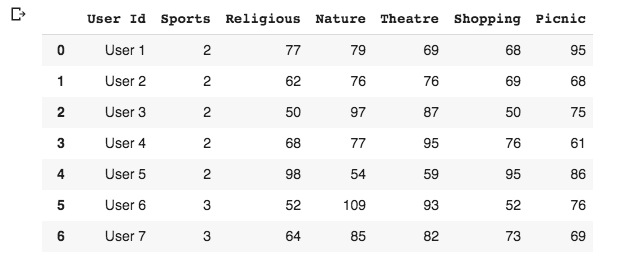
\includegraphics[width=1\textwidth]{Img/Review_dataset.png}
\caption{Review dataset activities}
\end{figure}

\clearpage
\subsubsection{KMeans}
In order to perform the clustering analysis we chose to set the number of clusters before the fit. K-means algorithm allowed us to follow this assumption. We applied the Elbow method to choose k. To get info about what activities customers did the most We followed two different paths: 

\paragraph*{Nature - Picnic}:
\begin{figure}[H]
\centering
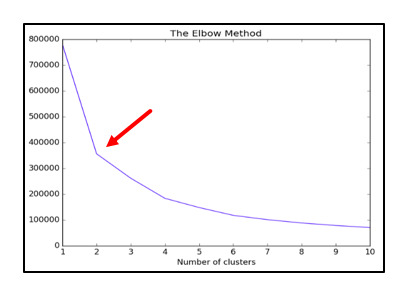
\includegraphics[width=0.6\textwidth]{Img/2_elbow.png}
\caption{Nature-Picnic Elbow method graph}
\end{figure}

\begin{figure}[H]
\centering
\hspace{-1cm}
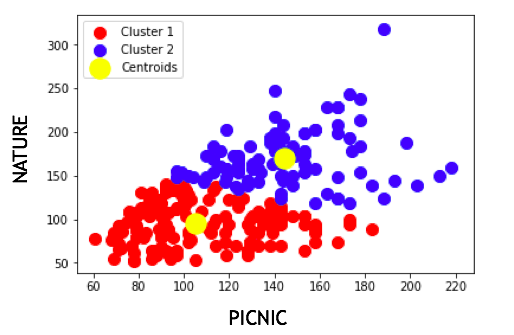
\includegraphics[width=0.8\textwidth]{Img/2_cluster.png}
	\caption{Nature-Picnic clustering}
\end{figure}
\noindent From the plot is clear that people did more picnics than nature activities, as the points are totally growing to the right. Recommending picnics on the app to natural people maybe would be a waste of time.
\clearpage

\paragraph*{Shopping - Nature}:
\begin{figure}[H]
\centering
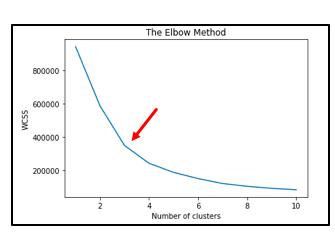
\includegraphics[width=0.7\textwidth]{Img/3_elbow.png}
\caption{Shopping-Nature Elbow method graph}
\end{figure}
\begin{figure}[H]
\centering
\hspace{-1.8cm}
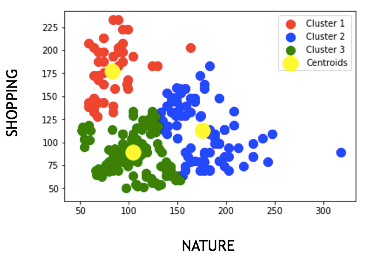
\includegraphics[width=0.8\textwidth]{Img/3_cluster.png}
\caption{Shopping-Nature clustering}
\end{figure}

\noindent The plot is very different from the previous one: it is reasonable to use three clusters as one of them is clearly apart. It is not easy to understand the correlation between the variables as people seem to behave very differently. Certainly shoppers don't normally go into the wild.
\clearpage

\subsubsection{Correlation Matrix}
In the end we realized that a clustering analysis was too much to be applied to this kind of dataset and it wasn't even giving us the kind of answers we were looking for. So we opted for a correlation matrix.

\begin{figure}[H]
\centering
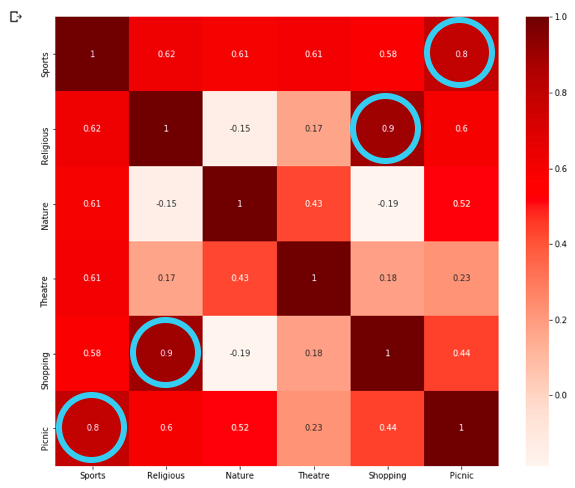
\includegraphics[width=1\textwidth]{Img/correlation_review.png}
\caption{Correlation matrix of the reviews}
\end{figure}

\noindent This type of plot let us understand if features are actually correlated or not. As seen in the clustering analysis, we have a 0.52 between nature and picnic, while shopping and nature are absolutely not linked at all (-0.19).\\
It's remarkable who Religion and Shopping also seem to be correlated at 0.9 out of 1, which it's quite surprising and unexpected.

\clearpage
\subsection{Classification}
The second insight we wanted to address was "Are we able to predict if the customer will return to the watershed after his first stay?".\\
In order to do that we used a Classification analysis and a particular dataset from the UCI repository. The dataset\footnote{\url{https://archive.ics.uci.edu/ml/datasets/Bank+Marketing}} is a (45211 x k) .csv file describing data related to a direct marketing campaigns of a Portuguese banking institution, based on phone calls. The campaign is divided in 3 steps (calls); our goal was to predict the customer behaviour at the end of the first call, without any data from the next calls. The final dataset, indeed, will be a (45211 x 9) .csv file.

\begin{itemize}
\item \textbf{Age}: age.
\item \textbf{Job}: type of job.
\item \textbf{Marital}: marital status.
\item \textbf{Education}: level of education.
\item \textbf{Default}: has credit in default?
\item \textbf{Balance}: balance of the year.
\item \textbf{Housing}: has housing loan?
\item \textbf{Loan}: has personal loan?
\item \textbf{y}: has the client subscribed a term deposit?
\end{itemize}

\noindent After the first stay of a customer, we assume to have available a similar dataset comprehensive of age, job, marital, education, in order to know if that customer will return or not.

\begin{figure}[H]
\centering
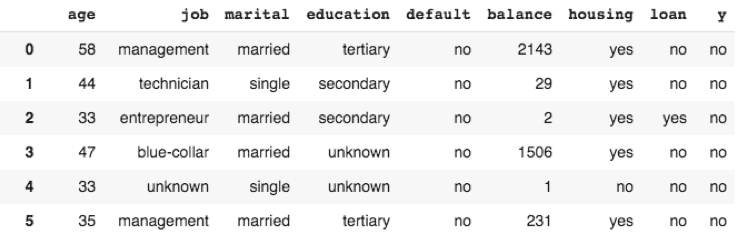
\includegraphics[width=1\textwidth]{Img/bank_dataset.png}
\caption{Customer dataset}
\end{figure}

\clearpage
\subsubsection{Feature Engineering}
Dealing with the second dataset required more data cleaning and engineering. First, we deleted all the next calls features, in order to cut all those information we couldn't use. Second we analyzed each variable one by one and decided how to encode it:
\begin{figure}[H]
\centering
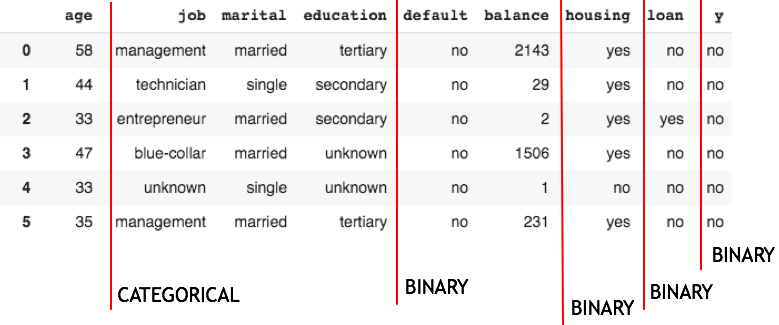
\includegraphics[width=0.8\textwidth]{Img/feature_recap.png}
\caption{Feature Engineering recap}
\end{figure}

\begin{itemize}[noitemsep]
\item \textbf{Education}: primary, secondary, tertiary (Label Encoded, since we want to keep track of the order. Tertiary brings higher value and score to the user).
\item \textbf{Marital}: married, single, divorced (binary modified, there's no need to introduce other categories).
\item \textbf{Default}: yes, no (binary).
\item \textbf{Housing}: yes, no (binary).
\item \textbf{Loan}: yes, no (binary).
\item \textbf{y}: yes, no (binary).

\begin{figure}[H]
\centering
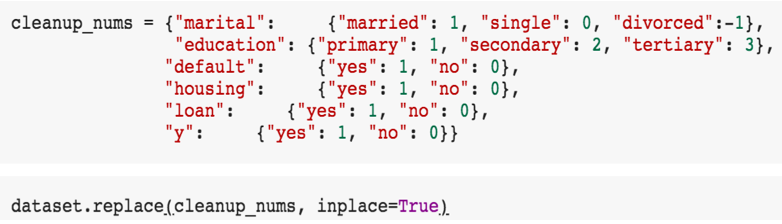
\includegraphics[width=0.7\textwidth]{Img/clean_up.png}
\caption{Cleanup}
\end{figure}
\item \textbf{Job}:  management, technician, etc (Categorical variable encoded as Dummy).
\begin{figure}[H]
\centering
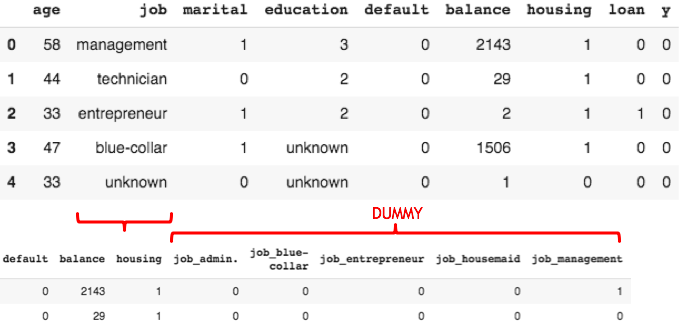
\includegraphics[width=0.6\textwidth]{Img/dummy.png}
\caption{Dummy encode}
\end{figure}
\end{itemize}

\subsubsection{Correlation Matrix}
Before any kind of analysis, we tried to understand feature correlation, in order to understand apriori if there were any dependencies. The matrix showed us there were no correlations at all.
\begin{figure}[H]
\centering
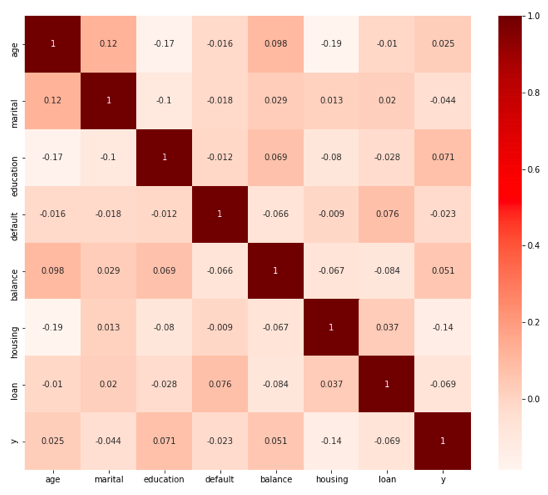
\includegraphics[width=0.6\textwidth]{Img/correlation_bank.png}
\caption{Correlation matrix of bank dataset}
\end{figure}
\vspace{-1cm}
\subsubsection{Metrics}
Since we were dealing with a classification problem, the first common solution we chose for metrics was confusion matrix, so that we could calculate accuracy and precision and use them to rate the models. During the process, however, we realized that we missed an important aspect of our dataset: the target, y, was imbalanced.
This event brought us to rethink our metrics and overall every consideration we were going to make. In the end we chose RECALL and F1 as main metrics, with a particular focus on RECALL as we want to identify the completeness of the classifier and lower as much as possible all the false negatives output, in order to focus on the customers who subscribed the service. 

\begin{figure}[H]
\centering
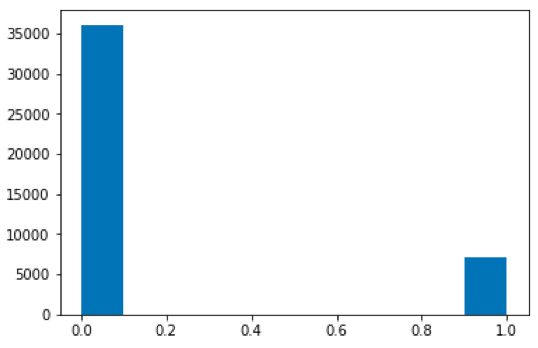
\includegraphics[width=0.7\textwidth]{Img/imbalanced.png}
\caption{Imbalanced metrics}
\end{figure}
\clearpage
\subsubsection{Models}
The second best way to solve a machine learning problem in general is to try several models and compare their results, as each model is characterized by unique features that, depending on the problem, are able to make it perform better or worse. This is specifically true for imbalanced dataset. In our analysis we focused on trees as decision trees frequently perform well on imbalanced data.
\\They work by learning a hierarchy of if/else questions that normally can be forced to address both classes.

\begin{itemize}
\item \textbf{Decision Tree Classifier}: DT seemed learning quite well from the dataset and, even if the recall was not so high, averall the F1 score was very curious.

\begin{figure}[H]
\centering
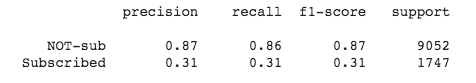
\includegraphics[width=0.7\textwidth]{Img/normal_tree.png}
\caption{Decision tree}
\end{figure}
\item \textbf{Random Forest Classifier}: as a generalization of decision tree, RF should have been performing better. On the contrary, during the process it had a different behavior. We'll discuss more about that after more analysis.

\begin{figure}[H]
\centering
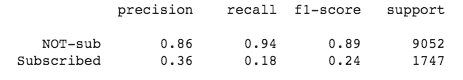
\includegraphics[width=0.7\textwidth]{Img/normal_forest.png}
\caption{Random forest}
\end{figure}

\item \textbf{K-NN}: Besides others, the third best one was the K-NN. We decided to put it into the documentation to proof the fact we considered also other kind of models, even if the result was worse.

\begin{figure}[H]
\centering
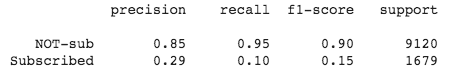
\includegraphics[width=0.7\textwidth]{Img/normal_knn.png}
\caption{K-NN}
\end{figure}
\end{itemize}

\noindent For any doubt, in the notebook each model has also it's confusion matrix, in order to make the reader understand better the overall trend.

\clearpage
\subsubsection{Under-Sampling}
Third way to address an imbalanced dataset is to re-sample specific features. In our case we lowered the number of rows of the biggest class. Under-sampling, in fact, can be defined as removing some observations from the majority class (the customer doesn't subscribe to the service or doesn't return to the watershed). 
The selection was performed completely randomly. The only drawback was that we were removing information that may be valuable. For the sake of simplicity (and not to bore the reader with hundreds on analysis) we will focus only on trees.

\begin{itemize}
\item \textbf{Decision Tree Classifier}: like in the case before, the highest subscribed recall score has been performed by a decision tree. Remarkable is the fact that the value almost doubled (0.65). 

\begin{figure}[H]
\centering
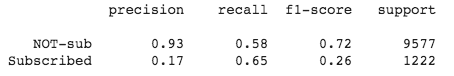
\includegraphics[width=0.7\textwidth]{Img/under_tree.png}
\caption{Under-Sampled decision tree}
\end{figure}
\item \textbf{Random Forest Classifier}: the greatest improvement, however, was performed by RF as from a very low 0.18 it reached 0.61 (lower than DT, but still very similar).

\begin{figure}[H]
\centering
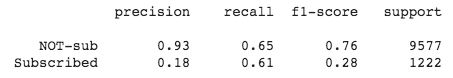
\includegraphics[width=0.7\textwidth]{Img/under_forest.png}
\caption{Under-Sampled random forest}
\end{figure}
\end{itemize}

\noindent F1 scores were slightly different from the normal case, but they were still keeping the small difference they had before. Between the two models, RF F1 did benefit the most from under-sampling.

\clearpage
\subsubsection{SMOTE}
In order to reach a complete overview of our analysis, we decided to apply another re-sampling technique, opposite from the first one, based on the concept of over sampling the minority dataset. Synthetic Minority Over-sampling Technique (SMOTE), in fact, is able to generate synthetic (fake) observations based on the real ones from the minor class, in order to reach a high similar volume of samples in both classes.

\begin{itemize}
\item \textbf{Decision Tree Classifier}: 

\begin{figure}[H]
\centering
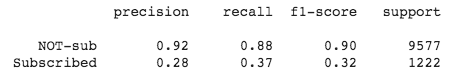
\includegraphics[width=0.7\textwidth]{Img/smote_tree.png}
\caption{SMOTE decision tree}
\end{figure}
\item \textbf{Random Forest Classifier}: 

\begin{figure}[H]
\centering
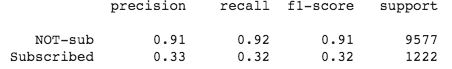
\includegraphics[width=0.7\textwidth]{Img/smote_forest.png}
\caption{SMOTE random forest}
\end{figure}
\end{itemize}

\noindent After the algorithm implementation, both models seemed to behave in a similar way. Precision and F1, in fact, were almost the same. RF, however, was the one which did benefit the most.
\clearpage
\subsection{Data Analysis Conclusion}
From a brute-force clustering attack we understood that a simple correlation matrix would have been more than fine to get the info we needed out of the dataset. It allowed us to understand connections we knew about (picnic - nature) and the ones we did not (shopping - religion).\\
The most challenging one has been the last analysis as we had to deal with an imbalanced dataset and decided to follow several paths. At first we studied the different metrics we could use to rate our results and recall was preferred. We then chose different models to use (decision tree and random forest were the best ones). At last we tried to re-sample our data and perform again each analysis.

\begin{itemize}
\item \textbf{Recall} 

\begin{figure}[H]
\centering
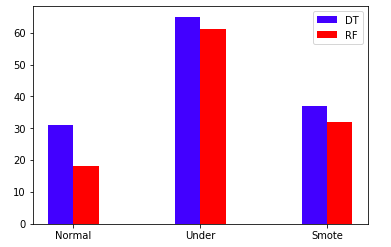
\includegraphics[width=0.6\textwidth]{Img/recall_recap.png}
\caption{Recall recap}
\end{figure}
\item \textbf{F1 score}: 

\begin{figure}[H]
\centering
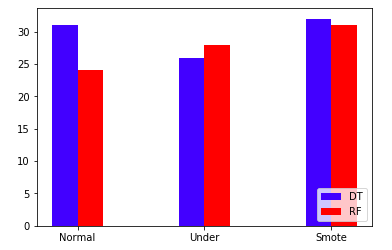
\includegraphics[width=0.6\textwidth]{Img/recap_f1.png}
\caption{F1 score recap}
\end{figure}
\end{itemize}

\noindent From the beginning we decided to use RECALL as main metric. It is clear that Decision Tree is overall the best model to address this dataset, that combined with the Under-sampling technique provided the best results.\\
However, considering the F1 score, it is interesting to notice how random forest model improved across the analysis and almost reached the same value as the decision tree, which, on the other hand, seems to behave totally fine even from the beginning, without any kind of sampling. This is maybe the proof that DT is effectively our best choice.